
%\section{Weakest Precondition Calculus} \label{wpGeneral}
This section describes the weakest precondition predicate transformer function which underlines the verification condition generator which will be presented later. 
The calculus is defined for the full Java sequential subset except for 64 bit data and floating point arithmetic and thus, deals with  object manipulation and creation,
 exception throwing and handling, subroutines. The weakest precondition predicate transformer understands the specification language BCSL. 
 

\subsection{Bytecode Programs. Background}\label{prelim}


In the following, we give a background information about programs written in our bytecode language and their  execution.
A Java bytecode program is a set of Java classes. Every Java class consists of a set of method declaration. 
Every method declaration (if not an abstract or interface method) 
has an array $\insOnly$ of bytecode instructions which constitute the method body.
The $k-th$ instruction in the bytecode array $\insOnly$ is  denoted with $\ins{k}$.
 We assume that the method bytecode has exactly one entry point
 (an entry point instruction is the instruction at which an execution of a method starts)
 and we denote it with $\entryPoint$.   If there is an execution path in which the instruction
 $\ins{j}$ may execute immediately after $\ins{k}$, we note it with $ \ins{k} \execRel \ins{j}$.

We assume that the control flow graph is reducible, i.e. every loop has exactly one entry point. This actually is admissible
as it is rarely the case that a compiler produce a bytecode with a non reducible flow graph and the practice shows that even hand written
code is usually reducible. Anyways, there are algorithms to transform a non reducible control flow graph to a reducible one. 
For more information on reducible flow graph, one can look at \cite{ARUCom1986}.
The next definition identifies backedges in the reducible control flow graph ( intuitively,  the edge that goes from 
from an instruction in a given loop in the control flow graph to the loop entry)  with the special execution relation $\execRel^l$ as follows:
 
\begin{defn}[Loop Definition]
\label{defLoop}
Let's have a bytecode program $\Pi$. We say that $\ins{e}$ is the entry instruction of loop $l$  and $\ins{f}$ is the end instruction
 of $l$ if and we note with
$ \ins{f} \execRel^l \ins{e}$ :
\begin{itemize}
\item every path in the control flow graph starting at the entry point $\entryPoint$  that reaches $\ins{f}$, passes through  $\ins{e}$ 
\item there is a path in which $\ins{e}$  is executed immediately after the execution of $\ins{f}$ ( $\ins{e} \execRel \ins{f}$)
\end{itemize}
\end{defn}


We illustrate the upper definitions with the control flow graph of the example from Fig.\ref{replaceSrc} in Fig. \ref{ctrlflow}.
In the figure we rather show the execution relation between basic blocks (a standard notion denoting a sequence of instructions where only the last one may be a 
jump and the first may be a target of a jump) the execution relation between the intstructions in a block being evident.


\begin{figure}[ht!]
\begin{center}
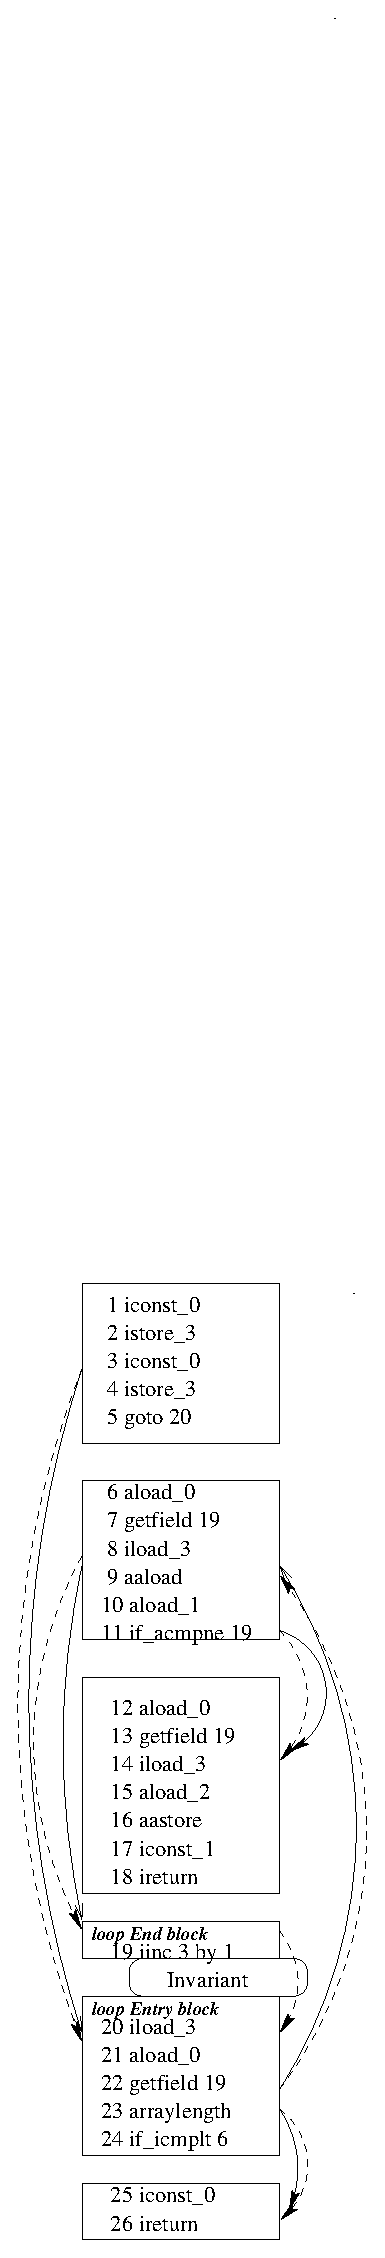
\epsfig{file=bytecode.eps, width=\linewidth}
\caption{The control flow graph of the source program from Fig.\ref{replaceSrc} }
\label{ctrlflow}
\end{center}
\end{figure}



\subsection{WP for a Java bytecode }\label{wp}
In what follows we assume that the bytecode has passed the bytecode verifier, thus it is well typed and well structured. Actually, our calculus is concerned 
with the program functional properties leaving the problem of code well structuredness and welltypedness to the bytecode verification techniques 


\subsubsection{Definitions} \label{wpHelp}
The predicate transformer function which for any instruction of the Java sequential fragment, depending
on the position of the instruction and on the function $\excPost$ determines the predicate that must hold in the prestate of the
instruction has the following signature :

$$ \fwpi : \tt{ instr} \longrightarrow  \tt{int} \longrightarrow ( int \longrightarrow  \tt{Exception}\longrightarrow  Predicate) \longrightarrow Predicate $$

The function  defined as follows :

$$ \excPostSpec_{\method} : \tt{ Exception  } \longrightarrow Predicate $$ 

returns the predicate that must hold if the method \method ends by throwing an exception 

The function $ \excPost(\tt{i}, \tt{Exc})$ where $i$ is an index in the bytecode of method \method is defined as follows:
\begin{itemize}
	\item it returns precondition  of the exception handler, if an exception handler that protects the instruction at index $i$ from exception of type \texttt{Exc } exists
	\item otherwise it is equal to $\excPostSpec_{\method}( \tt{Exc})$
\end{itemize}

Also, every time an exception of type \texttt{E} is thrown a new object of type  \texttt{E} is allocated on the heap $\heap \oplus [ \reference{E} \longrightarrow  \tt{obj(E, f)}]  $ and the reference $\reference{E}$ is put on the stack top. 

We denote the postcondition of a method with $ \normalPost$.
\textit{Note:} In what follows we ignore the  Java error exceptions. Thus we deal only with user defined exceptions and
 \texttt{JavaRuntimeException} subclasses


First we define the function $inter$ that for two instructions that may execute one 
after another in some execution graph determines the predicate $ \inter(k,j)$ the predicate that must hold in between them. This 
definition determines if at a given program point there is an invariant to hold or it is the precondition of the next instruction to hold.

\begin{defn}[intermediate predicate between two instructions  ]\label{inter}
Assume that $\ins{k} \execRel \ins{j}$. The predicate $\inter{k}{ j}$ must hold after the execution of $\ins{k}$ and before the execution of 
$\ins{j}$ and is defined as follows:
\begin{itemize}
\item if  $\ins{k} \execRel^l \ins{j}$
then the corresponding loop invariant must hold:
$$
\inter{k}{j} =  \invariant
$$

\item else if $\ins{j}$ is a loop entry then the corresponding loop invariant $\invariant$ must hold before $\ins{j}$ is executed, 
i.e. after the execution of $\ins{k}$. We also require that \invariant \ implies the weakest precondition of the loop entry instruction. 
The implication is quantified over the locations $m_i , i= 1..s$ that may be modified in the loop.

$$
\inter{k}{j}= \invariant \ \wedge \ \forall_{i = 1..s} m_i.(
\invariant \Rightarrow \wpi{\ins{j}}{j}{ \excPost })
$$
\item else 
$$
\inter{k}{j} = \wpi{ \ins{j} }{j}{\excPost}
$$
\end{itemize}
\end{defn}




 
\subsubsection{Weakest Precondition Calculus Rules} \label{wprules}

We now define the rules for the predicate transfomer \textrm{wp} for our bytecode programming language

\begin{itemize}	
\item Control transfer instructions
\begin{enumerate}
 \item unconditional jumps \\
$$\wpi{\instr{goto \  n}}{i} {\excPost} =   \inter{i}{n}$$

\item conditional jumps

$\wpi{\instr{if\_cond  \  n}}{i} {\excPost} =$
$$ \left\{ \begin{array}{l} 
 \texttt{cond}( \stack{\counter}, \stack{\counter - 1} ) \Rightarrow \ \inter{i}{n}[\counter \leftarrow \counter - 2 ] \\
  \wedge  \\
 not( \texttt{cond}( \stack{\counter},\stack{\counter - 1} ))  \Rightarrow \ \inter{i}{i+1}[\counter \leftarrow \counter - 2 ] \\
  \end{array}
\right.
 $$


 \item return 
 
 $\wpi{\instr{return}}{i} {\excPost}  = \normalPost[ \backslash result \leftarrow \stack{\counter}]$

\end{enumerate}


\item subroutines\\
Subroutines are treated by inlining, thus every the precondition of every jsr instruction depends on the subroutine code which is executed after it.
\begin{enumerate}

\item $ \wpi{\instr{jsr \ n}}{i}{\excPost} =  \inter{i}{n} $\\

\item$ \wpi{\instr{ret \ n}}{i}{\excPost} =  \inter{i}{k} $
for any instruction $\ins{k}$ which follows a \texttt{jsr} instruction, that jumps to the subroutine ending with $\ins{i}$
\end{enumerate}


\item  load and store instructions
	\begin{enumerate}
		\item load \\
		 $\wpi{\instr{load } \ j} {i} {\excPost}  = $ \\
		 $ \inter{i}{i+1}[\counter \leftarrow \counter   +1][  \stack{ \counter  + 1} \leftarrow \register{j}  ]$ \\
		
		\item store	 \\	 
		$\wpi{\instr{store } \ j} {i} {\excPost}  =   $ \\ 
	$	\inter{i}{i+1}[\counter \leftarrow \counter   - 1][  \register{j} \leftarrow \stack{ \counter }   ]$ \\
		
		\item push  \\
			$\wpi{\instr{push } \ j} {i} {\excPost}  =   $ \\ 
	$	\inter{i}{i+1}[\counter \leftarrow \counter   + 1][  signExtendToInt(j) \leftarrow \stack{ \counter +1 }   ]$ \\
		
		The value $\texttt{j}$, which is of type $\texttt{byte}$  in the case push = \instr{bipush} and is of type $\texttt{short}$  in case 
		push = \instr{sipush}. It is sign extended to int  before pushed on the stack. 
	
	     % \item iconst\_j   (j = -1, 0, 1, 2, 3, 4 or 5)  \\
		%			$\wpi{\instr{iconst}\_j} {i} {\excPost}  =   $ \\ 
			%		$	\inter{i}{i+1}[\counter \leftarrow \counter   + 1][  j \leftarrow \stack{ \counter +1}   ]$ \\

		\item iinc 
				$\wpi{\instr{iinc } \ j} {i} {\excPost}   = $ \\
				$ \inter{i}{i+1}[ \register{j} \leftarrow \register{j} + 1   ] $
		  
	\end{enumerate}
	
\item arithmetic instructions
	\begin{enumerate}
		\item instruction that cannot  cause exception throwing    (\texttt{arithOp} =  \instr{add}, \instr{sub}, \instr{mult}, 
				\instr{and}, \instr{or}, \instr{xor} , \instr{ishr}, \instr{ishl},     )\\
				$\wpi{\instr{arithOp}} {i} {\excPost}   = $ \\
				$ \inter{i}{i+1}[\counter \leftarrow \counter   - 1][ \stack{\counter - 1} \leftarrow  \stack{\counter} \ \texttt{op} \ \stack{\counter -1}   ] $

	
						
		\item instructions that may throw exceptions ( \texttt{arithOp} =  \instr{rem}, \instr{div} )\\
				$\wpi{\instr{arithOp } } {i} {\excPost}  =$
				$$\left\{
				\begin{array}{l}
				 \stack{\counter} \neq \Mynull \Rightarrow \\
				  \Myspace  \inter{i}{i+1} [\counter \leftarrow \counter   - 1] \\
				\Myspace \Myspace  \Myspace    	[ \stack{\counter - 1} \leftarrow  \stack{\counter} \ \texttt{op}  \ \stack{\counter -1}] \\
				\wedge \\
				\stack{\counter} = \Mynull \Rightarrow  \\
				\Myspace \Myspace  \excPost(i,\tt{ArithmeticExc})[\counter \leftarrow 0] \\
				\Myspace \Myspace \substitution{\heap}{\heap[\oplus \Ref{ArithmeticExc } \longrightarrow \objCl{ArithmeticExc}]}\\
				
				\Myspace \Myspace    [ \stack{0} \leftarrow  \reference{ArithmeticExc}] \\
				\end{array} \right.
				$$
	\end{enumerate}
%	\item conversion instructions( i2b, i2s, i2c). Only the cases for the instruction  i2b is considered, the others being similar 
%		\begin{itemize}
	%			\item   i2b   \\
	%			$\wpi{\instr{i2b } } {i} {\excPost}  = \inter{ i} {i+1} [\stack{\counter} \leftarrow  signExtendToInt(\stack{\counter} \& \& 0xFF)] $
				
	%	\end{itemize}
		
\item  object creation and manipulation 
	\begin{enumerate}
		\item new \\
		$\wpi{\instr{new  \ Class}} {i} {\excPost}  = $ \\
		$$ \begin{array}{l} 
		\inter{i}{i+1} [ \counter \leftarrow \counter + 1 ] \\
		\Myspace [ \stack{ \counter + 1} \leftarrow \reference{Class}  ] \\
		\Myspace [ \heap  \leftarrow \heap[\oplus  \reference{Class} \longrightarrow \objCl{Class} ]]
		\end{array}
		$$
		\heap \ is updated with the newly created object and a reference to it is put on the top of the stack: \\
	
		
		\item array creation
		
	         %  either \texttt{instr } = \instr{newarray}  and \texttt{type} is a basic type ( int), \\
				 % either  \texttt{instr } =  \instr{anewarray}  and type is a reference type\\
				 $\wpi{\instr{newarray  \ type}} {i} {\excPost}  = $ \\
					$$
					\begin{array}{l}
					\stack{\counter} \ge 0 \Rightarrow  \\
						\Myspace  \Myspace \inter{i}{i+1} [ \heap  \leftarrow \heap[\oplus  \Ref{type} \longrightarrow \objCl{type,\stack{\counter} }]\\
								\Myspace	[\stack{\counter} \leftarrow \Ref{type}]  \\
							\wedge \\
						\stack{\counter} < 0 \Rightarrow  \\
							 
						\Myspace  \Myspace  \excPost( i, \tt{ NegativeArraySizeExc}) \\
                                            	\Myspace  \Myspace  \substitution{\heap}{\heap[\oplus \Ref{NegativeArraySizeExc } \longrightarrow \objCl{NegativeArraySizeExc }]}\\
						\Myspace  \Myspace  [\counter \leftarrow 0] \\
						\Myspace  \Myspace  [\stack{0} \leftarrow  \reference{ NegativeArraySizeExc}]
						\end{array} 
					$$ where a newly created object $\texttt{obj(type, \stack{\counter}}$ is allocated in the \heap \  
and a  reference $\reference{type}$  \ to it is put on the stack top $ \heap = \heap[\oplus  \reference{type} \longrightarrow \texttt{obj(type, \stack{\counter}}]$
			%	\item   $\wpi{\instr{multinewarray  \ Class \ dims}} {i} {\excPost}  = $ \\
				%	$$
					%	\begin{array}{l}o
						% \end{array} 
				%	$$
		
			\item getfield \\
				 $\wpi{\instr{getField  \ f }} {i} {\excPost}  = $ \\
				 $$
						\begin{array}{l}
							\stack{\counter } \ne \Mynull \Rightarrow \\
									 \inter{i}{i+1}[ \stack{\counter } \leftarrow \tt{f}( \stack{\counter } ) ] \\
									 \wedge \\
								\stack{\counter } = \Mynull \Rightarrow \\
								\Myspace  \Myspace   \excPost( i, \tt{ NullPointerExc}) \\
								 \Myspace  \Myspace \Myspace  \substitution{\heap}{\heap[\oplus \Ref{NullPointerExc} 
							\longrightarrow \objCl{NullPointerExc}]}\\
								\Myspace  \Myspace  [\counter \leftarrow 0] \\	
								\Myspace  \Myspace  \Myspace    [\stack{0} \leftarrow  \reference{ NullPointerExc}]
	  
						\end{array} 
					$$
			\item  putfield \\
			$\wpi{\instr{putField  \ f }} {i} {\excPost}  = $ \\
				 $$
						\begin{array}{l}
							\stack{\counter } \ne \Mynull \Rightarrow \\
									 \inter{i}{i+1} [ \counter \leftarrow  \counter -2  ] \\
									 \Myspace[ \tt{f}  \leftarrow  \tt{f} (\oplus [ \stack{\counter - 2}  \longrightarrow  \stack{\counter  -1} ] ) ] \\
									 \wedge \\
								\stack{\counter } = \Mynull \Rightarrow \\
								\Myspace  \Myspace  \Myspace  \excPost( i, \tt{ NullPointerExc}) \\
								 \Myspace  \Myspace \Myspace \Myspace  \Myspace  \substitution{\heap}{\heap[\oplus \Ref{NullPointerExc} 
							\longrightarrow \objCl{NullPointerExc}]}\\
								\Myspace  \Myspace  \Myspace   \Myspace  \Myspace  [\counter \leftarrow 0] \\
								\Myspace  \Myspace  \Myspace   \Myspace  \Myspace   [\stack{0} \leftarrow  \reference{ NullPointerExc}]
	  
						\end{array} 
					$$
					\item arraylength  - returns the length of the array which is on the  top of the stack \\
					$\wpi{\instr{arraylength  \ f }} {i} {\excPost}  = $ \\
					 $$
						\begin{array}{l}
							\stack{\counter } \ne \Mynull \Rightarrow \\
									 \inter{i}{i+1}
									 \Myspace[ \stack{\counter }  \leftarrow  length(\stack{\counter } )  ] \\
									 \wedge \\
								\stack{\counter } = \Mynull \Rightarrow \\
								\Myspace  \Myspace  \excPost( i, \tt{ NullPointerExc}) \\
								\Myspace  \Myspace  \Myspace    [\counter \leftarrow 0] \\
								\Myspace  \Myspace  \Myspace   [\stack{0} \leftarrow  \reference{ NullPointerExc}]
	  
						\end{array} 
					$$
					\item checkcast 
						$\wpi{\instr{checkcast  \ Class}} {i} {\excPost}  = $ \\
						$$
						\begin{array}{l}
							subtype( getType(\stack{\counter}),  \tt{Class } ) \vee  \stack{\counter} = \Mynull \Rightarrow \\
									 \inter{i}{i+1}\\
									 \wedge \\
								not( subtype( getType(\stack{\counter}),  \tt{Class } )) \Rightarrow \\
								\Myspace  \Myspace   \excPost( i, \tt{ ClassCastExc}) \\
								\Myspace  \Myspace  \Myspace  \substitution{\heap}{\heap[\oplus \Ref{NullPointerExc} \longrightarrow \objCl{NullPointerExc}]}\\
								\Myspace  \Myspace  \Myspace    [\counter \leftarrow 0] \\
								\Myspace  \Myspace  \Myspace    [\stack{\counter} \leftarrow  \reference{ClassCastExc}]
	  
						\end{array} 
					$$
						\item instanceof
						$\wpi{\instr{instanceof  \ Class}} {i} {\excPost}  = $ \\
						$$
						\begin{array}{l}
							subtype(getType(\stack{\counter}),  \tt{Class } )  \Rightarrow \\
									 \inter{i}{i+1}[ \stack{\counter }  \leftarrow 1  ] \\
									 \wedge \\
								not( subtype( getType(\stack{\counter}),  \tt{Class } ))  \vee  \stack{\counter} = \Mynull \Rightarrow \\
								 \inter{i}{i+1} [ \stack{\counter }  \leftarrow 0 ] \\	  
						\end{array} 
					$$
	\end{enumerate}
%	\item Stack management
%		         \begin{itemize}
%						 \item pop  \\
%	  							$\wpi{\instr{pop}} {i} {\excPost}  =  \inter{i}{i+1}[ \counter \leftarrow \counter -1]$ \\
%%	  					\item dup \\
%	  							$$
%	  							\begin{array}{l}\wpi{\instr{dup}} {i} {\excPost}  =  \inter{i}{i+1}[ \counter \leftarrow \counter + 1] \\
%	  							\Myspace \Myspace \Myspace \Myspace \Myspace   [ \stack{\counter + 1} \leftarrow  \stack{\counter}]
%	  							 \end{array}
%	  							 $$
%	 				 	\item swap 
%	 				 			$\wpi{\instr{swap}} {i} {\excPost}  =  $ \\
%	 				 			$$ 
%	 				 			\begin{array}{l}
%	 				 					\inter{i}{i+1}[  \stack{\counter} \leftarrow var ] \\
%	 				 						\Myspace \Myspace \Myspace [  \stack{\counter + 1} \leftarrow  \stack{\counter}  ] \\
%	 				 						\Myspace \Myspace \Myspace [  var  \leftarrow  \stack{\counter + 1}  ] \\
%	 				 			\end{array}
%	 				 			$$ \\
%\end{itemize} 
	 				 	\item method invocation  (only the case for non void instance method is given). We take into account the normal and abnormal termination cases
	 				 	for the method invocation.  The rules states that the precondition of the called method must be established; 
	 				 	the postcondition of the called method is assumed to hold. \\
	 				 			$\wpi{\instr{invoke  \   m}} {i} {\excPost}  =  $ \\
	 				 			$$ 
	 				 			\begin{array}{l}
	 				 			pre( \texttt{m})[ \register{s} \leftarrow \stack{\counter + s - numargs(m)}]_{s = 0}^{numargs(m) }  \\
	 				 			\wedge \\
	 				 			\forall  \tt{e_m} ( m =1 .. k  )(  \\ 
	 				 				post( \texttt{m} )[\result \leftarrow freshVar ]\\
	 				 				\Myspace \Myspace [ \register{s} \leftarrow \stack{\counter + s - numargs(m)}]_{s = 0}^{numargs(m) } \\	 				 						\Myspace  \Myspace  \substitution{\heap}{\heap[\oplus \Ref{Cl_s } \longrightarrow \objCl{Cl_s}]_{s=0}^t}\\
	 				 					 \Myspace \Myspace \Rightarrow \\  
	 				 					\Myspace \Myspace \Myspace  \inter{i}{i+1 } [\counter \leftarrow \counter -  \tt{numargs(m)}   ] \\ 
										\Myspace \Myspace \Myspace \Myspace   [  \stack{\counter -  numargs(m)   } \leftarrow freshVar ]																																										
	 				 			) \\
	 				 			\wedge_{j = 1}^s \\
	 				 			\forall \tt{e_m} ( m =1 .. k  ) ( \excPost^{\texttt{m}}( \tt{Exc_j} ) \Rightarrow   \excPost(i,\tt{Exc_j})  ) \\		
	 				 			\end{array}
	 				 			$$ \\
	 				 		$ \tt{Exc_j} , j = 1 .. s$ the exceptions that the method \texttt{m } may throw \\ \\
	 				 		$	\excPost^{\tt{m} }$ the function which returns the predicate $	\excPost^{\tt{m} }(\tt{Exc})$ that holds
	 				 		if the exception \texttt{Exc} is thrown.\\  \\
							$ \excPost( i, \reference{Exc_j}) $ is the either the precondition of the exception handler protecting
							from exceptions of type $\tt{Exc_j}$ at index $i$ or is the exceptional postcondition $excPost( \tt{Exc_j} )$ 
							if such an exception handler does not exist \\	\\
	 				 		$pre( \tt{m})$ - the precondition of method \texttt{m} \\ \\
	 				 		$ post( \texttt{m} )$ - the postcondition of method \texttt{m} \\ \\
	 				 		$\tt{e_m}( m =1 .. k  )  $ - the locations that may be modified by method  \texttt{m}  \\ \\
							also the rule reflects that in the heap may have been allocated new objects during the execution of the invoked method
						

\item throw exception instruction \\
				
							$ \wpi{\instr{athrow }} {i} {\excPost}  =$
							$$ \begin{array}{l} 
								\stack{\counter} \neq \Mynull \Rightarrow  \excPost( i, \stack{\counter}) \\
								\wedge \\
								\stack{\counter} = \Mynull \Rightarrow  \excPost( i, \reference{NullPointerExc}) \\
							   \end{array}
							$$ \\
						The thrown object is on the top of the stack, and that is why the precondition of the \instr{athrow } instruction  
						depends on \stack{\counter}.
						
	 			
\end{itemize}



\subsection{Example}

\subsubsection{Weakest Precondition in the Presence of Loop }
The following example shows how the weakest precondition calculus is applied to the example program for which we have shown the source code at Fig. \ref{replaceSrc} and
 its bytecode control flow graph at Fig. \ref{ctrlflow}. 
In particular, the example that comes here after 
gives the weakest preconditions  for the instructions that are part  of the loop of the method body. 
Thus, every instruction is preceded with its weakest precondition enclosed in curly braces.
The invariant is written at the place where it must hold (i.e. where the backedge relating the loop entry and the loop end is). The weakest precondition of every instruction is calculated w.r.t.
 the weakest precondition of the next instruction in the execution path. So,
 looking at the example, the precondition of instruction $19$ is calculated w.r.t. the loop 
invariant.  The weakest precondition of the instruction $18$ is calculated w.r.t. the wp of instruction $19$ etc. Also the wp of the jump instruction $24$ is calculated from the weakest 
precondition of instruction $6$. 
This example shows the process of calculating the verification conditions for a program. 

 The wp of a method body is the conjunction the wps  of all of its execution paths. 

$$
\begin{array}{l}
 % \tt{ 1 \ iconst\_0 } \\

 % \tt{ 2 \ istore\_3 } \\

 % \tt{ 3 \ iconst\_0 } \\

 % \tt{ 4 \ istore\_3 } \\



 % \tt{ 5 \ goto \ 20 } \\

\ldots \\

\\
  \{ \\
 \locVar{0} = \Mynull \Rightarrow \false  \wedge\\ 
 \locVar{0} \neq \Mynull \Rightarrow \\
 \Myspace 	test.ListArray.list(\locVar{0} ) \neq \Mynull \wedge \\ 
 \Myspace 	len(test.ListArray.list(\locVar{0} ) ) > \locVar{3} \wedge \\ 
 \Myspace 	\locVar{3} \geq 0 \wedge \\   
 \Myspace 	\locVar{1} \neq ListArray.list(\locVar{0})[\locVar{3} ]  \Rightarrow  \\ 
 \Myspace \Myspace     1 + \locVar{3}  \leq len(test.ListArray.list(\locVar{0}))  \wedge \\
 \Myspace \Myspace     1 + \locVar{3}  \geq 0 \wedge \\ 
 \Myspace \Myspace   \forall  var(0).   0 \leq var(0) \wedge var(0) < 1 + \locVar{3}   \Rightarrow  \\ 		             
 \Myspace \Myspace \Myspace  ListArray.list(\locVar{0} )[var(0)] \neq \locVar{1}        \\
		\wedge \\
ListArray.list(\locVar{0} ) = \Mynull  \Rightarrow  \false   \wedge \\
  len(test.ListArray.list(\locVar{0})) \le \locVar{3} \vee \locVar{3} < 0 \Rightarrow  \false  \\
\}  \\
\bf{ 6 \ aload\_0 }\\
\\


  \{ \\
\stack{\counter} =  \Mynull \Rightarrow \false  \wedge \\ 
 \stack{ \counter} \neq \Mynull \Rightarrow \\
 \Myspace 	ListArray.list(\stack{\counter}) \neq \Mynull  \wedge \\ 
 \Myspace        len(test.ListArray.list(\stack{\counter})) > \locVar{3} \wedge  \\
 \Myspace 	\locVar{3} >= 0   \wedge \\
 \Myspace 	\locVar{1} \neq ListArray.list(\stack{\counter})[\locVar{3}]   \Rightarrow \\
 \Myspace \Myspace 	1 + \locVar{3} <= len(test.ListArray.list(\locVar{0})) \wedge \\
 \Myspace \Myspace 	1 + \locVar{3} >= 0  \wedge \\
 \Myspace \Myspace 	\forall  var(0). \  0 \leq var(0) \wedge var(0) < 1 + \locVar{3}  \Rightarrow \\
 \Myspace \Myspace \Myspace ListArray.list(\locVar{0})[var(0)] \neq \locVar{1}   \wedge \\
ListArray.list(\stack{\counter}) = \Mynull \Rightarrow \false   \wedge \\
  len(test.ListArray.list(\stack{\counter})) <= \locVar{3} \vee \locVar{3} < 0  \Rightarrow \false \\
\}  \\
\bf{ 7 \ getfield \ ListArray.list} \\

\end{array}$$
$$
\begin{array}{l}
\\
\{ \\
 \stack{\counter} \neq \Mynull \wedge \\ 
 len(\stack{\counter}) > \locVar{3} \wedge \\
 \locVar{3} \geq 0 \wedge \\
 \locVar{1} \neq \stack{\counter}[\locVar{3}]  \Rightarrow \\
 \Myspace 	1 + \locVar{3} \leq len(ListArray.list(\locVar{0})) \wedge \\
 \Myspace 		1 + \locVar{3} >= 0  \wedge \\
 \Myspace 		\forall  var(0)  . 0 <= var(0) \wedge (var(0) < 1 + \locVar{3} \Rightarrow \\
 \Myspace   \Myspace  ListArray.list(\locVar{0})[var(0)] \neq \locVar{1}   \wedge \\
 \stack{\counter} = \Mynull) \Rightarrow \false \wedge \\
  len(\stack{\counter}) \leq \locVar{3} \vee \locVar{3} < 0  \Rightarrow \false  \\
\}\\ 
\bf{ 8 \ iload\_3} \\




\\
\{ \\
 \stack{\counter - 1} \neq \Mynull \wedge \\ 
   len(\stack{\counter - 1} > \stack{\counter}  \wedge \\ 
   \stack{\counter} \geq 0  ) \wedge \\
     \locVar{1} \neq \stack{\counter - 1}[\stack{\counter}] \Rightarrow \\ 
  \Myspace                1 + \locVar{3} \leq len(test.ListArray.list(\locVar{0})) \wedge \\ 
\Myspace 		 1 + \locVar{3} \geq 0  \wedge \\
\Myspace 		 \forall  var(0). \   0 \leq var(0) \wedge var(0) < 1 + \locVar{3}  \Rightarrow \\ 
		\Myspace 	\Myspace \Myspace 	 ListArray.list(\locVar{0})[var(0)] \neq \locVar{1}  \wedge \\ 
\stack{\counter - 1} = \Mynull) \Rightarrow \false   \wedge  \\
len(\stack{\counter - 1}) \leq \stack{\counter} \vee \stack{\counter} < 0 \Rightarrow \false \\  
\}\\ 
\bf{ 9 \ aaload} \\


\\
\{ \\ 
  \locVar{1} \neq \stack{\counter} \Rightarrow  \\
 \Myspace   1 + \locVar{3} \leq len(test.ListArray.list(\locVar{0}) \wedge \\ 
 \Myspace  1 + \locVar{3} \geq 0 \wedge \\ 
  \Myspace \forall  var(0)  . \   0 \leq var(0) \wedge var(0) < 1 + \locVar{3}  \Rightarrow  ListArray.list(\locVar{0})[var(0)] \neq \locVar{1}  \\ 
\} \\
 
\bf{10 \ aload\_1} \\ 

\\
\{ \\
\stack{\counter} \neq \stack{\counter -1} \Rightarrow \\ 
\Myspace  1 + \locVar{3} \leq len(test.ListArray.list(\locVar{0})) \wedge \\
\Myspace  1 + \locVar{3} \geq 0 \wedge  \\
\Myspace  \forall  var(0). \ 0 \leq var(0) \wedge var(0) < 1 + \locVar{3} \Rightarrow   \\
 \Myspace \Myspace   ListArray.list(\locVar{0})[var(0)] \neq \locVar{1} \\
\} \\
 \bf{11 \ if\_acmpne 19 } \\
 
\end{array}$$

$$
\begin{array}{l}
\ldots \\ 
% 12 \ aload\_0 \\
% 13 \ getfieldListArray.list \\
% 14 \ iload\_3 \\
% 15 \ aload\_2 \\
% 16 \ aastore \\
% 17 \ iconst\_1
% 18 \ ireturn \\
\ldots \\
\\
\{ \\
   1 + \locVar{3} \leq len(test.ListArray.list(\locVar{0}))) \wedge \\
   1 + \locVar{3} \geq 0 \wedge  \\
\forall  var(0). \ 0 \leq var(0) \wedge var(0) < 1 + \locVar{3} \Rightarrow   \\
\Myspace ListArray.list(\locVar{0})[var(0)] \neq \locVar{1}   \\
\} \\

\bf{ 19 \ iinc  \ 3  } \\

\\
\{ \\
\bf{invariant :}\\ 
   \locVar{3} \leq len(test.ListArray.list(\locVar{0})) \wedge \\
   \locVar{3} \geq 0 \wedge  \\
\forall  var(0). \ 0 \leq var(0) \wedge var(0) < \locVar{3} \Rightarrow   \\
\Myspace ListArray.list(\locVar{0})[var(0)] \neq \locVar{1}   \\
\} \\


\\

\{ \\
 \forall  var(27). \   var(27) \neq \locVar(0)  \wedge \\ 
 \forall  var(26) .\ var(26) \geq 0 \wedge var(26) < len(test.ListArray.list(var(27)) \Rightarrow \\ 
 \Myspace ListArray.list(var(27))[var(26)] =ListArray.list\_at\_20(var(27))[var(26)]  \wedge \\ 
 \Myspace \locVar{3}\_at\_20 \leq len(ListArray.list\_at\_20(\locVar{0})) \wedge \\ 
 \Myspace \locVar{3}\_at\_20 \geq 0  \wedge \\ 
 \Myspace \forall  var(0). \  0 \leq var(0) \wedge var(0) < \locVar{3}\_at\_20  \Rightarrow \\ 
\Myspace \Myspace ListArray.list\_at\_20(\locVar{0})[var(0)] \neq \locVar{1} 

\\    \Rightarrow \\ 

 \Myspace  \locVar{0} = \Mynull \Rightarrow \Myfalse  \wedge\\
 \Myspace  \locVar{0} \neq \Mynull \Rightarrow \\ 
 \Myspace  \Myspace ListArray.list\_at\_20(\locVar{0}) \neq \Mynull \wedge \\ 
 \Myspace  \Myspace  \locVar{3}\_at\_20) < len( ListArray.list\_at\_20(\locVar{0})) \Rightarrow \\ 
 \Myspace  \Myspace \Myspace  \locVar{0} = \Mynull \Rightarrow \Myfalse  \wedge \\ 
 \Myspace  \Myspace \Myspace  \locVar{0} \neq \Mynull \Rightarrow  \\
  \Myspace  \Myspace \Myspace \Myspace ListArray.list\_at\_20(\locVar{0}) \neq \Mynull \wedge \\ 
  \Myspace  \Myspace \Myspace \Myspace len(ListArray.list\_at\_20(\locVar{0}))
 > \locVar{3}\_at\_20 \wedge \\
\Myspace  \Myspace \Myspace \Myspace  \locVar{3}\_at\_20 \geq 0   \wedge \\ 
\Myspace  \Myspace \Myspace \Myspace  \locVar{1} \neq ListArray.list\_at\_20(\locVar{0})[\locVar{3}\_at\_20]  \Rightarrow \\ 
\Myspace  \Myspace \Myspace \Myspace \Myspace  1 + \locVar{3}\_at\_20 \leq 
len(test.ListArray.list\_at\_20(\locVar{0})) \wedge \\ 
\Myspace  \Myspace \Myspace \Myspace \Myspace 1 + \locVar{3}\_at\_20 \geq 0  \wedge \\ 
\Myspace  \Myspace \Myspace \Myspace \Myspace \forall  var(0) . 0 \leq var(0)) \wedge  var(0) < 1 + \locVar{3}\_at\_20  \Rightarrow \\ 
\Myspace  \Myspace \Myspace \Myspace \Myspace \Myspace ListArray.list\_at\_20)(\locVar{0})[var(0)] \neq \locVar{1}  \wedge \\  
\Myspace  \Myspace \Myspace \Myspace \Myspace
 ListArray.list\_at\_20(\locVar{0}) = \Mynull \Rightarrow \Myfalse  \wedge \\ 
\Myspace  \Myspace \Myspace \Myspace \Myspace len(test.ListArray.list\_at\_20)(\locVar{0}) \leq \locVar{3}\_at\_20 \vee \locVar{3}\_at\_20 < 0 \Rightarrow \Myfalse ) ) \\ 
\} \\
\bf{20 \ aload\_3} \\



\end{array}
$$

$$
\begin{array}{l}
\{\\
  \locVar{0} = \Mynull \Rightarrow \Myfalse  \wedge \\
  \locVar{0} \neq \Mynull \Rightarrow \\ 
  \Myspace ListArray.list(\locVar{0}) \neq \Mynull \wedge \\ 
  \Myspace \stack{\counter - 1} < len(test.ListArray.list(\locVar{0})  \Rightarrow \\  
  \Myspace \locVar{0} = \Mynull \Rightarrow  \Myfalse  \wedge \\ 
  \Myspace \locVar{0} \neq  \Mynull \Rightarrow \\  
  \Myspace \Myspace  ListArray.list(\locVar{0}) \neq \Mynull \wedge \\ 
  \Myspace \Myspace  len(test.ListArray.list(\locVar{0})) > \locVar{3} \wedge \\ 
  \Myspace \Myspace \locVar{3} \geq 0  ) \wedge \\ 
  \Myspace \Myspace \locVar{1} \neq  ListArray.list(\locVar{0})[\locVar{3}] \Rightarrow \\  
  \Myspace \Myspace \Myspace  1 + \locVar{3} \leq len(test.ListArray.list(\locVar{0})) \wedge \\ 
  \Myspace \Myspace \Myspace  1 + \locVar{3} \geq 0  \wedge \\ 
  \Myspace \Myspace \Myspace \forall  var(0). \ 0 \leq var(0) \wedge var(0) < 1 + \locVar{3}  \Rightarrow \\  
   \Myspace \Myspace \Myspace \Myspace ListArray.list(\locVar{0})[var(0)] \neq \locVar{1} ) ) ) \wedge \\ 
 \Myspace ListArray.list(\locVar{0}) = \Mynull \Rightarrow  \Myfalse  \wedge \\ 
 \Myspace len(test.ListArray.list(\locVar{0})) \leq \locVar{3}) \vee (\locVar{3} < 0)  \Rightarrow  \Myfalse ) )  \wedge \\ 
 \Myspace ListArray.list(\locVar{0}) = \Mynull) \Rightarrow  \Myfalse  \\
\} \\

 \bf{21 \ aload\_0} \\

 \\

\{\\
  \stack{\counter} = \Mynull \Rightarrow \Myfalse  \wedge \\
  \stack{\counter} \neq \Mynull \Rightarrow \\ 
  \Myspace ListArray.list(\stack{\counter}) \neq \Mynull \wedge \\ 
  \Myspace \stack{\counter - 1} < len(test.ListArray.list(\stack{\counter})  \Rightarrow \\  
  \Myspace \locVar{0} = \Mynull \Rightarrow  \Myfalse  \wedge \\ 
  \Myspace \locVar{0} \neq  \Mynull \Rightarrow \\  
  \Myspace \Myspace  ListArray.list(\locVar{0}) \neq \Mynull \wedge \\ 
  \Myspace \Myspace  len(test.ListArray.list(\locVar{0})) > \locVar{3} \wedge \\ 
  \Myspace \Myspace \locVar{3} \geq 0  ) \wedge \\ 
  \Myspace \Myspace \locVar{1} \neq  ListArray.list(\locVar{0})[\locVar{3}] \Rightarrow \\  
  \Myspace \Myspace \Myspace  1 + \locVar{3} \leq len(test.ListArray.list(\locVar{0})) \wedge \\ 
  \Myspace \Myspace \Myspace  1 + \locVar{3} \geq 0  \wedge \\ 
  \Myspace \Myspace \Myspace \forall  var(0). \ ( ( (0 \leq var(0)) \wedge (var(0) < (1 + \locVar{3})) ) \Rightarrow \\  
   \Myspace \Myspace \Myspace \Myspace ListArray.list(\locVar{0})[var(0)] \neq \locVar{1} ) ) ) \wedge \\ 
 \Myspace ListArray.list(\locVar{0}) = \Mynull \Rightarrow  \Myfalse  \wedge \\ 
 \Myspace len(test.ListArray.list(\locVar{0})) \leq \locVar{3}) \vee (\locVar{3} < 0)  \Rightarrow  \Myfalse ) )  \wedge \\ 
 \Myspace ListArray.list(\stack{\counter}) = \Mynull) \Rightarrow  \Myfalse  \\
\} \\
\bf{22 \ getfield \ ListArray.list} \\


\end{array}
$$

$$
\begin{array}{l}
\{ \\
\stack{\counter} = \Mynull \Rightarrow \Myfalse \\
 \stack{\counter} \neq \Mynull  \wedge \\ 
 \stack{\counter - 1} < len(\stack{\counter}) \Rightarrow \\
 \Myspace  \locVar{0} = \Mynull \Rightarrow \Myfalse  \wedge \\ 
 \Myspace  \locVar{0} \neq \Mynull  \Rightarrow  \\
 \Myspace  \Myspace  ListArray.list(\locVar{0}) \neq \Mynull \wedge \\ 
 \Myspace  \Myspace  len(test.ListArray.list(\locVar{0})) > \locVar{3} \wedge \\
 \Myspace  \Myspace  \locVar{3} \geq  0  \wedge \\
 \Myspace  \Myspace  \locVar{1} \neq ListArray.list(\locVar{0}[\locVar{3}] )  \Rightarrow \\ 
 \Myspace  \Myspace \Myspace  1 + \locVar{3} \leq len(test.ListArray.list(\locVar{0})) \wedge \\ 
 \Myspace  \Myspace \Myspace  1 + \locVar{3} \geq 0  \wedge  \\
 \Myspace  \Myspace \Myspace  \forall  var(0). \  0 \leq var(0) \wedge var(0) < 1 + \locVar{3}  \Rightarrow \\
 \Myspace  \Myspace \Myspace \Myspace ListArray.list(\locVar{0})[var(0)] \neq \locVar{1}   )  ) ) \wedge \\ 
 \Myspace  ListArray.list(\locVar{0}) = \Mynull) \Rightarrow \Myfalse  \wedge  \\
 \Myspace  len(test.ListArray.list(\locVar{0})) \leq \locVar{3}) \vee \locVar{3} < 0 \Rightarrow \Myfalse \\
\} \\ 
\bf{23 \ arraylength} \\

\\

\{ \\
 \stack{\counter - 1} < \stack{\counter} \Rightarrow \\
 \Myspace  \locVar{0} = \Mynull \Rightarrow \Myfalse  \wedge \\ 
 \Myspace  \locVar{0} \neq \Mynull  \Rightarrow  \\
 \Myspace  \Myspace   ListArray.list(\locVar{0}) \neq \Mynull \wedge \\ 
 \Myspace  \Myspace   len(test.ListArray.list(\locVar{0})) > \locVar{3} \wedge \\
 \Myspace  \Myspace   \locVar{3} \geq  0  \wedge \\
 \Myspace  \Myspace    \locVar{1} \neq ListArray.list(\locVar{0}[\locVar{3}] )  \Rightarrow \\ 
 \Myspace  \Myspace \Myspace  1 + \locVar{3} \leq len(test.ListArray.list(\locVar{0})) \wedge \\ 
 \Myspace  \Myspace \Myspace  1 + \locVar{3} \geq 0  \wedge  \\
 \Myspace  \Myspace \Myspace  \forall  var(0). \  0 \leq var(0) \wedge var(0) < 1 + \locVar{3}  \Rightarrow \\
 \Myspace  \Myspace \Myspace \Myspace ListArray.list(\locVar{0})[var(0)] \neq \locVar{1}   )  ) ) \wedge \\ 
 \Myspace  ListArray.list(\locVar{0}) = \Mynull) \Rightarrow \Myfalse  \wedge  \\
 \Myspace  len(ListArray.list(\locVar{0})) \leq \locVar{3}) \vee \locVar{3} < 0 \Rightarrow \Myfalse \\
\} \\
 \bf{24 \  if\_icmplt 6 }\\



\end{array}$$


\subsection{Correctness}

The correctness criteria for the \textrm{wp} calculus requires that if the function is applied to a bytecode program \texttt{P} and postcondition $\psi^{post}$ ,
 predicate calculated by the calculus is provable  then if  the postcondition upon which 
